\section{Motivation}
\label{s:motivation}

% - characteristics of concurrency bugs
% - challenges / design requirements
% - limitations of existing approaches


\dr{TODO: muzz, conzzer}
%
This work is motivated by an observation that none of previous works
properly addresses characteristics of \textit{offending thread
  interleaving} (\ie, one that causes a concurrency bug).
%
As a consequence, previous works either \textbf{1)} are not able to
identify whether offending thread interleaving remains
untested~\cite{krace}, or \textbf{2)} waste the computing power by
executing too many redundant instances of thread
interleaving~\cite{snowboard, razzer}.


In this section, we first comprehend why concurrency bugs manifest
depending on thread interleaving through a real-world concurrency bug
example.
%
We then define design goals to effectively discover concurrency bugs
in the kernel, and summarize why existing approaches fall short in
satisfying the design goals.


\PP{Manifestation of concurrency bugs}
%
\begin{figure}[t]
  \centering
  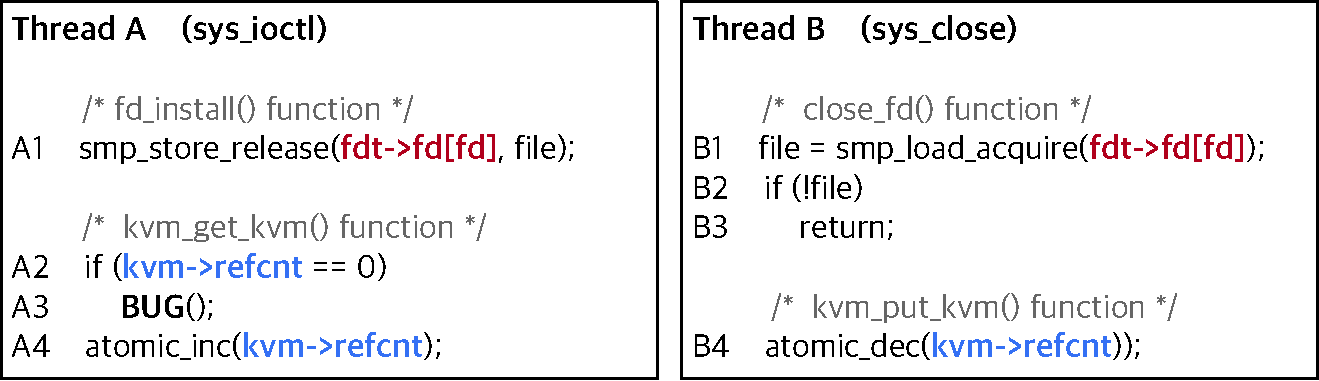
\includegraphics[width=0.95\linewidth]{fig/cve-2017-10661.pdf}
  \caption{Simplified code snippet of CVE-2017-7533. If \texttt{B1} is
    executed between \texttt{A2} and \texttt{A4}, a concurrency bug on
    \texttt{inet->hdrincl} leads to uninitialized stack pointer usage
    on \texttt{rfv}, and an attacker may gain root privileges.}
  \label{fig:cve-2019-6974}
\end{figure}
%
\autoref{fig:cve-2019-6974} describes how an erroneous instance of
thread interleaving causes a concurrency bug.
%
In this example, an uninitialized access bug may manifest when two
system calls are executed concurrently: \texttt{sendmsg()} to send a
message through an ipv4 socket, and \texttt{setsockopt()} to modify an
option of the ipv4 socket. As a consequence of the uninitialized
access bug, an attacker may gain root privileges.



Assuming \texttt{inet->hdrincl} is initially \texttt{1}, the
concurrency bug manifests depending on the execution order of three
memory accesses, \texttt{A2} and \texttt{A4} in thread~A, and
\texttt{B1} and in thread~B.
%
During sending a message through the ipv4 socket, thread~A reads a
value of \texttt{inet->hdrincl} twice at \texttt{A2} and \texttt{A4}.
%
However, since these two read operations are not atomically executed,
thread~B may intervene in the middle of these two read operations.
%
In that case, if \texttt{B1} is executed between \texttt{A2} and
\texttt{A4}, thread~A reads different values of \texttt{inet->hdrincl}
at \texttt{A2} and \texttt{A4}, and dereference \texttt{rfv} without
initializing it.


This example indicates that the manifestation of a concurrency bug
depends on the execution order of multiple memory
accesses. Specifically, a concurrency bug is \textit{a combined result
  of a few scheduling constraints}, where each scheduling constraint
is established on a pair of memory accesses.
%
In this example, \texttt{rfv} is not initialized only if \texttt{A2}
is executed before \texttt{B1}. Thus, the uninitialized access
requires a scheduling constraint
$\texttt{A2} \Rightarrow \texttt{B1}$~\footnote{In this paper,
  $\texttt{X} \Rightarrow \texttt{Y}$ denotes that \texttt{X} is
  executed before \texttt{Y}}.
%
Similary, a scheduling constraint on \texttt{B1} and \texttt{A4} is
also required for the concurrency bug to manifest since thread~A
dereferences uninitialized \texttt{rfv} only if
$\texttt{B1} \Rightarrow \texttt{A4}$.
%
In summary, among all possible instances of thread interleaving, only
ones that \textit{conjunctively satisfy the two scheduling
  constraints, \ie,
  $(\texttt{A2} \Rightarrow \texttt{B1}) \wedge (\texttt{B1}
  \Rightarrow \texttt{A4})$}, cause the concurrency bug while and all
other interleaving instances cannot.

\PP{Design goals}
%
The main goal of this paper is to design a fuzzing technique to
effectively discover kernel concurrency bugs. To this end, we identify
two design goals of a concurrency fuzzer as follows:

\begin{enumerate}[label=\textbf{R\arabic*:}]
%
\item \emph{A fuzzer should be able to determine that offending
  thread interleaving remains untested.}
\item \emph{A fuzzer should be able to quickly explore untested
    offending thread interleaving.}
%
\end{enumerate}

For example in \autoref{fig:cve-2019-6974}, \textbf{R1} states that a
fuzzer should adopt a proper interleaving coverage metric that can be
used to determine whether
$(\texttt{A2} \Rightarrow \texttt{B1}) \wedge (\texttt{B1} \Rightarrow
\texttt{A4})$ remains untested or not, and \textbf{R2} emphasizes an
importance of a scheduling mechanism that quickly covers this
conjunctive condition instead of exploring the entire search space of
thread interleaving.



\subsection{Limitation of prior approaches}
\label{ss:existingapproaches}

Even though prior approaches achieve their own successes, none of them
satisfy \textbf{R1} and \textbf{R2}.

\PP{Insufficient coverage metric}
%
\begin{figure}[t]
  \centering
  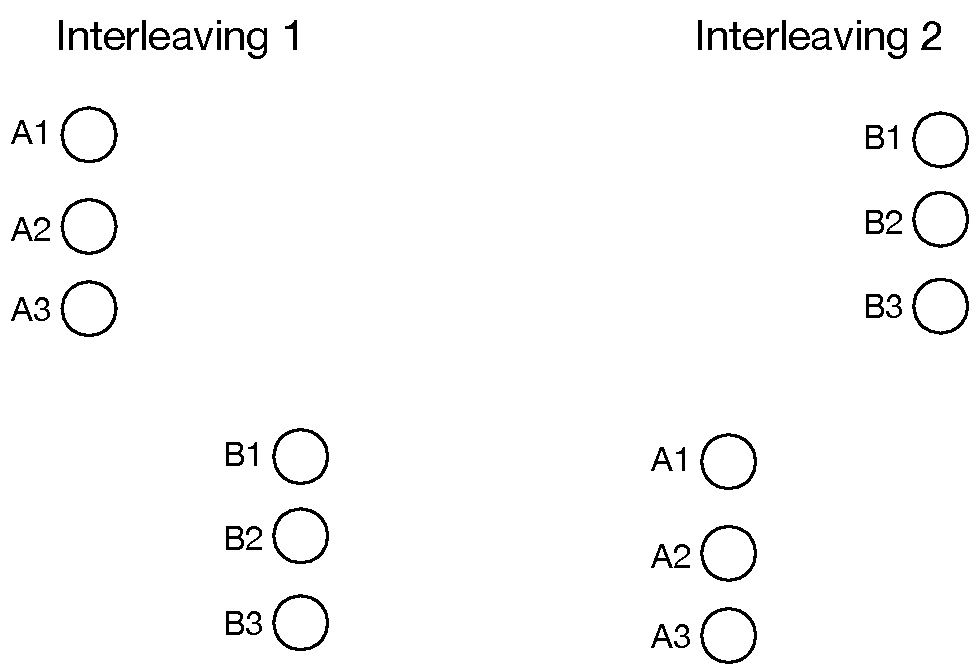
\includegraphics[width=0.95\linewidth]{fig/alias-coverage.pdf}
  \caption{Two instances of thread interleaving between thread~A and
    thread~B described in \autoref{fig:cve-2019-6974}. Regarding
    \texttt{inet->hdrincl}, alias coverage is saturated but the
    concurrency bug doest not manifest.}
  \label{fig:alias-coverage}
\end{figure}
%
To the best of our knowledge, existing concurrency coverage metrics
are not sufficient to determine whether interesting (\ie, offending)
thread interleaving remains untested. Thus, they do not satisfy
\textbf{R1}.
%
In particular, after KRace~\cite{krace} first emphasizes the necessity
of a coverage metric in the concurrency dimension, different
concurrency coverage metrics are proposed such as \textit{alias
  coverage}~\cite{krace}, \textit{concurrent call
  pair}~\cite{conzzer}, and \textit{\dr{TODO: MUZZ
    coverage}}~\cite{muzz}.
%
However, they are not applicable to track behavioral changes according
to a combination of scheduling constraints, mainly because they either
track only a \textit{single} scheduling constraint~\cite{krace, muzz}
or \textit{coarse-grained information} such as a pair of two
concurrently-executed functions~\cite{conzzer}.

Taking the example of alias covarege, \autoref{fig:alias-coverage}
describes two interleaving instances that saturate alias coverage
found between two system calls in \autoref{fig:cve-2019-6974}.
%
In these example interleaving scenarios, the uninitialized access does
not manifest even after alias coverage is saturated, and a fuzzer may
decide to stop searching for new interleaving instances in the two
system calls.
%
While we do not enumerate all proposed interleaving coverage metrics
here, we find that they all share the same limitation.


\PP{Ineffective scheduling mechanism}
%
Stemming from insufficient coverage metrics, proposed scheduling
mechanisms are also ineffective in satisfying \textbf{R2}.
%
As described in \autoref{s:background}, proposed scheduling mechanisms
are largely categorized into two: a randomized scheduler and a
hint-directed scheduler.

\dr{revisit after evaluation. not ready to write this part:}
%
Randomized schedulers~\cite{krace, pctalgorithm, muzz, ski} pay little
attention on collected interleaving coverage when scheduling
instructions, and rely on the randomness in diversifying thread
interleaving.
%
Therefore, they are inherently limited in satisfying a specific
condition of thread interleaving (\eg,
$(\texttt{A2} \Rightarrow \texttt{B1}) \wedge (\texttt{B1} \Rightarrow
\texttt{A4})$ in \autoref{fig:cve-2019-6974}).
%
This limitation is even more pronounced by a recent study,
ExpRace~\cite{exprace}, stating that many concurrency
bugs~\cite{cve20196974, cve20191999, cve201911486} manifest only if
thread interleaving satisfies an extreme condition that randomized
scheduler hardly satisfy.
%
Unfortunately, ExpRace demonstrates that this kind of concurrency bugs
are equally threatening the security of the kernel.


Whereas, % hint-directed schedulers~\cite{razzer, snowboard} enforce
% thread interleaving, and thus, are able to deterministically trigger
% concurrency bugs, even those that manifest under an extreme condition
% of thread interleaving.
% %
% However, 
state-of-the-art approaches adopting a hint-directed
scheduler, Razzer~\cite{razzer} and Snowboard~\cite{snowboard}, are
not capable of diversifying thread interleaving across iterations.
%
Since they do not adopt interleaving coverage, they are not able to
determine which thread interleaving requires further
testing. Therefore, they vary thread interleaving a small degree
across fuzzing iterations, and require a long time to trigger
concurrency bugs.
%
According to our evaluation~\autoref{s:eval}, ...


% In the perspective of fuzzing, a coverage metric is a paramount gear
% to determine whether a given input is worthy of further mutation.
% %
% If a coverage metric does not represent whether an input has a
% potential to trigger a race condition, a fuzzer may ignore inputs in
% which there are unexplored interleavings, or waste the computing power
% to valueless inputs.
% %
% In this regard, our primary question is whether existing coverage
% metrics in the concurrency dimension are suitable to apprehend
% interleavings potentially causing a race condition, for example,
% $(\texttt{A1} \Rightarrow \texttt{B1}) \wedge (\texttt{B4} \Rightarrow
% \texttt{A2})$ in \autoref{fig:cve-2019-6974}.



% Unfortunately, we observe that none of existing approaches incorporate
% a proper coverage metric for race conditions.
% %
% A few of existing approaches~\cite{snowboard, razzer} do not adopt a
% coverage in the concurrency dimension at all. Therefore, they do not
% make a decision as to whether a given input is worth further testing.
% %
% Other approaches~\cite{krace, muzz} adopt coverage metrics that are
% not suitable for race conditions as they do not consider a combined
% result of multiple pairs of conflicting accesses. As a consequence,
% race conditions may not be exposed even after the coverages are
% saturated.
% %
% % Consequently, existing approaches have difficulty in distinguishing a
% % given input has a potential to cause an interesting behavior, \ie,
% % a race condition.



% \yj{This is the key paragraph to point out the limitation of previous approaches, but very vague. Make specific claims of why Kraces' alias coverage is insufficient by giving an example.}
% %
% In order to show why comprehending multiple pairs of conflicting
% accesses is important, let us suppose we have three inputs that
% consists of two concurrent syscalls as described in
% \autoref{fig:alias-coverage}.
% %
% For all inputs, thread~A executes a \texttt{mmap()} syscall to map the
% binder driver to a user address space while thread~B handles different
% ioctl requests such that \texttt{ioctl(FREE_BUFFER)},
% \texttt{ioctl(REPLY)}, and \texttt{ioctl(TRANSACTION)} for
% \texttt{Input 1}, \texttt{Input 2}, and \texttt{Input 3} respectively.
% %
% It is worth noting that in \texttt{Input 1} and \texttt{Input 2},
% there is only one pair of conflicting accesses; in \texttt{Input 1},
% the two threads conflict on \texttt{alloc->vma}, and in \texttt{Input
%   2}, the two threads conflict on \texttt{alloc->mm}.



% \begin{figure}[t]
%   \centering
%   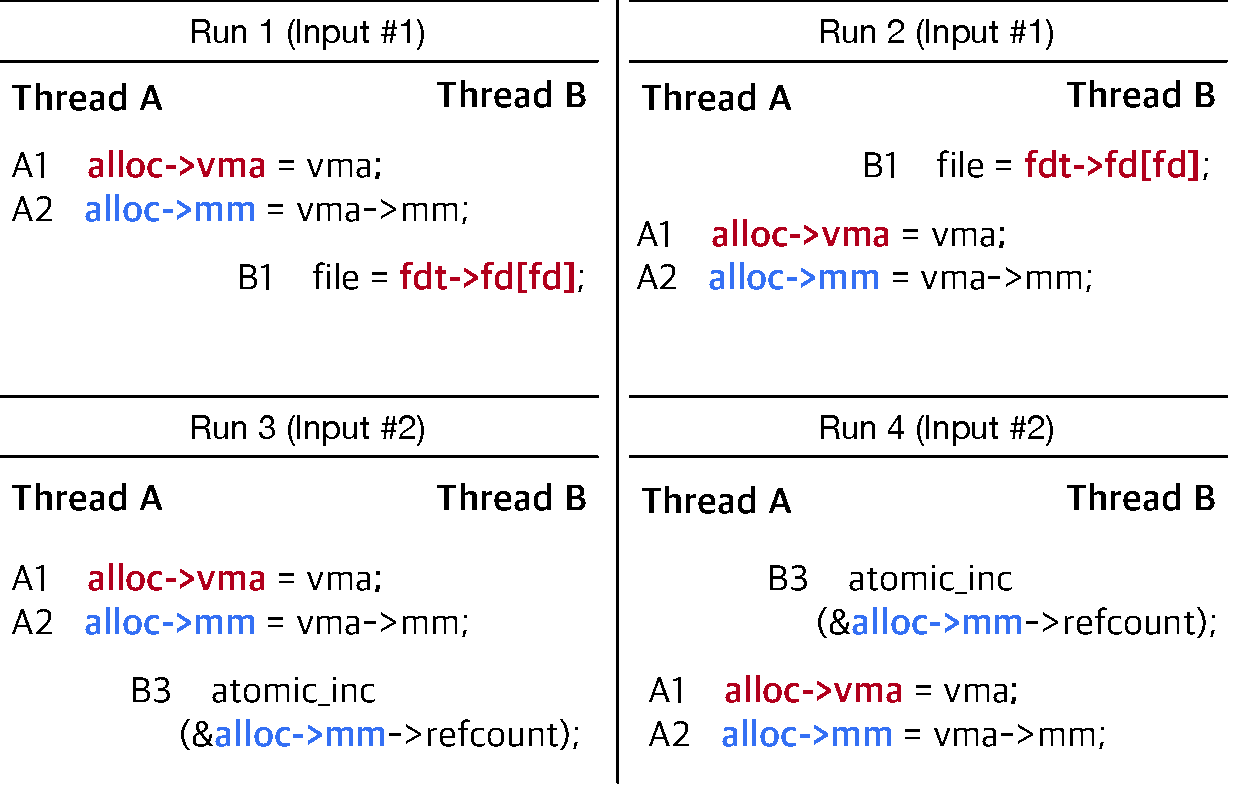
\includegraphics[width=0.9\linewidth]{fig/alias-coverage-interleaving.pdf}
%   \caption{Four interleavings of \texttt{Input 1} and \texttt{Input 2}
%     in \autoref{fig:alias-coverage}. After executing these four
%     interleavings, all possible execution orders of a single
%     conflicting accesses are exhibited.\dr{Run 1 -> Interleaving 1?}}
%   \label{fig:alias-coverage-interleaving}
% \end{figure}

% In this example, if we adopt a coverage metric that focuses on a
% single pair of conflicting accesses (\eg, alias coverage), a fuzzer
% may not recognize that \texttt{Input 3} may exhibit a different
% behavior than \texttt{Input 1} and \texttt{Input 2}~(\ie, a
% NULL-dereference bug).
% %
% \autoref{fig:alias-coverage-interleaving} shows four interleavings
% that exhibits all execution order of a single pair of conflicting
% accesses. If a fuzzer executes \texttt{Input 1} with interleavings in
% \texttt{Run 1} and \texttt{Run 2}, a fuzzer observes execution orders
% such as $\texttt{A1} \Rightarrow \texttt{B1}$ (in \texttt{Run 1}) and
% $\texttt{B1} \Rightarrow \texttt{A1}$ (in \texttt{Run 2}).
% %
% Similary, if a fuzzer executes \texttt{Input 2} with interleavings in
% \texttt{Run 3} and \texttt{Run 4}, it observes execution orders of
% $\texttt{A2} \Rightarrow \texttt{B4}$ (in \texttt{Run 3}) and
% $\texttt{B4} \Rightarrow \texttt{A2}$ (in \texttt{Run 4}).
% %
% After executing these four interleavings, \texttt{Input 3} does not
% reveal a new execution order of a single conflicting
% accesses. Therfore, as a Krace state, a fuzzer may de-prioritize
% \texttt{Input 3}, and the race condition may not be found.

% In summary, in order to determine whether an input shows interesting
% behaviors or not, a fuzzer needs to comprehend \textit{a combined
%   result of multiple pairs of conflicting accesses} as it is the
% primary reason of race conditions.



%%% Local Variables:
%%% mode: latex
%%% TeX-master: "p"
%%% End:
